\documentclass{sigchi-ext}
% Please be sure that you have the dependencies (i.e., additional
% LaTeX packages) to compile this example.
\usepackage[T1]{fontenc}
\usepackage{textcomp}
\usepackage[scaled=.92]{helvet} % for proper fonts
\usepackage{graphicx} % for EPS use the graphics package instead
\usepackage{balance}  % for useful for balancing the last columns
\usepackage{booktabs} % for pretty table rules
\usepackage{ccicons}  % for Creative Commons citation icons
\usepackage{ragged2e} % for tighter hyphenation
\usepackage{todonotes} % the notes to self

% Some optional stuff you might like/need.
% \usepackage{marginnote} 
% \usepackage[shortlabels]{enumitem}
% \usepackage{paralist}
% \usepackage[utf8]{inputenc} % for a UTF8 editor only

%% EXAMPLE BEGIN -- HOW TO OVERRIDE THE DEFAULT COPYRIGHT STRIP --
% \copyrightinfo{Permission to make digital or hard copies of all or
% part of this work for personal or classroom use is granted without
% fee provided that copies are not made or distributed for profit or
% commercial advantage and that copies bear this notice and the full
% citation on the first page. Copyrights for components of this work
% owned by others than ACM must be honored. Abstracting with credit is
% permitted. To copy otherwise, or republish, to post on servers or to
% redistribute to lists, requires prior specific permission and/or a
% fee. Request permissions from permissions@acm.org.\\
% {\emph{CHI'14}}, April 26--May 1, 2014, Toronto, Canada. \\
% Copyright \copyright~2014 ACM ISBN/14/04...\$15.00. \\
% DOI string from ACM form confirmation}
%% EXAMPLE END

% Paper metadata (use plain text, for PDF inclusion and later
% re-using, if desired).  Use \emtpyauthor when submitting for review
% so you remain anonymous.
\def\plaintitle{
XRAY: Inspector Tools For Designers
} 
\def\plainauthor{First Author, Second Author, Third Author,
% Fourth Author, Fifth Author, Sixth Author
  }
\def\emptyauthor{}
\def\plainkeywords{Authors' choice; of terms; separated; by
  semicolons; include commas, within terms only; required.}
\def\plaingeneralterms{Documentation, Standardization}

\title{XRAY: Inspector Tools For Designers} 


\numberofauthors{6}
% Notice how author names are alternately typesetted to appear ordered
% in 2-column format; i.e., the first 4 autors on the first column and
% the other 4 auhors on the second column. Actually, it's up to you to
% strictly adhere to this author notation.
\author{%
  \alignauthor{%
    \textbf{First Author}\\
    \affaddr{University of Author} \\
    \affaddr{Authortown, CA 94022, USA} \\
    \email{author1@anotherco.edu} }\alignauthor{%
    \textbf{Second Author}\\
    \affaddr{YetAuthorCo, Inc.}\\
    \affaddr{Authortown, BC V6M 22P Canada}\\
    \email{author5@anotherco.com} } \vfil \alignauthor{%
    \textbf{Third Author}\\
    \affaddr{VP, Authoring}\\
    \affaddr{Authorship Holdings, Ltd.}\\
    \affaddr{Awdur SA22 8PP, UK}\\
    \email{author2@author.ac.uk} }
    % \alignauthor{%
    % \textbf{Sixth Author}\\
    % \affaddr{Universit\'e de Auteur-Sud}\\
    % \affaddr{40222 Auteur France}\\
    % \email{author6@author.fr} } \vfil \alignauthor{%
    % \textbf{Third Author}\\
    % \textbf{Fourth Author}\\    
    % \affaddr{L\={e}khaka Interaction Labs}\\
    % \affaddr{Bengaluru 560 080, India}\\
    % \email{author3@anotherco.com} \\
    % \email{author4@hchi.anotherco.com} }\alignauthor{%
    % \textbf{Seventh Author}\\
    % \affaddr{Department of Skrywer}\\
    % \affaddr{University of Umbhali}\\
    % \affaddr{Cape Town, South Africa}\\
    % \email{author7@umbhaliu.ac.za} } 
    }

% Make sure hyperref comes last of your loaded packages, to give it a
% fighting chance of not being over-written, since its job is to
% redefine many LaTeX commands.
\definecolor{linkColor}{RGB}{6,125,233}
\hypersetup{%
  pdftitle={\plaintitle},
%  pdfauthor={\plainauthor},
  pdfauthor={\emptyauthor},
  pdfkeywords={\plainkeywords},
  bookmarksnumbered,
  pdfstartview={FitH},
  colorlinks,
  citecolor=black,
  filecolor=black,
  linkcolor=black,
  urlcolor=linkColor,
  breaklinks=true,
}

% \reversemarginpar%

\begin{document}

%% For the camera ready, use the commands provided by the ACM in the Permission Release Form.
%\CopyrightYear{2007}
%\setcopyright{rightsretained}
%\conferenceinfo{WOODSTOCK}{'97 El Paso, Texas USA}
%\isbn{0-12345-67-8/90/01}
%\doi{http://dx.doi.org/10.1145/2858036.2858119}
%% Then override the default copyright message with the \acmcopyright command.
%\copyrightinfo{\acmcopyright}

\maketitle

% Uncomment to disable hyphenation (not recommended)
% https://twitter.com/anjirokhan/status/546046683331973120
\RaggedRight{} 

% Do not change the page size or page settings.
\begin{abstract}
Examples, both in the form of web templates and snippets of code, are widely used in the creation of websites. Numerous tools have been created to facilitate developer's borrowing of code from live websites and galleries. 
These include in-browser developer tools, firebug, and other tools. However, little exploration has been done on the experience of designers working on partially-developed or live sites. This paper introduces XRAY, inspector tools for designers, which allow the designer to adjust fonts, colors, margins, and padding without ever needing to look at HTML or CSS. These features were designed to increase experimentation by automating consistency (percolating changes), making this technical, code-based task more approachable for designers by creating a UI similar to (??) instead of traditional inspector tools, and improving designer-developer communication by allowing designers to export a document with all changes in a format that developers will be comfortable with. Moreover, XRAY 
promotes the use of design systems by only suggesting styling options that exist in the current design system and highlighting where current aesthetics violate the design system. Our user study showed that experienced designers were xx\% more efficient and yy\% more successful when they used xray than the standard industry tools. 
\end{abstract}

\keywords{\plainkeywords}

\category{H.5.m}{Information interfaces and presentation (e.g.,
  HCI)}{Miscellaneous}\category{See}{\url{http://acm.org/about/class/1998/}}{for
  full list of ACM classifiers. This section is required.}

\section{Introduction}
Both programmers and web designers look at websites for design inspiration and at snippets of code for guidance. Researchers and industry professionals have made developers tools to enable these programmers and designers to learn more from these examples. However, many of these tools are geared towards those who are comfortable with code. 

Currently, the status quo is (explain how it works for most designers). (Most designers use tools and processes like these to tweak existing websites (markup in sketch, emails, meeting in person, etc). 

We contribute XRAY, design tools for developers, a set of novel design tools that allow the designer to adjust fonts, colors, margins, and padding without ever needing to look at HTML or CSS. 

These features were designed to increase experimentation by automating consistency (percolating changes), making this technical, code-based task more approachable for designers by creating a UI similar to (??) instead of traditional inspector tools, and improving designer-developer communication by allowing designers to export a document with all changes in a format that developers will be comfortable with. 
First, increase experimentation by: 
\begin{itemize}
    \item 
    % \item [Learn from others / Increase consistency / Speedup making changes] 
    
    % Allows designer to copy styles from other elements. 
    % \item [Developer / Designer communication] 
    
    % Keep track of all changes made and produce a document that can be given to a programmer detailing all changes. Track all changes
    % \item[Developer / Designer communication] 
    
    % Reduce the barrier for designers to make style changes on live websites. (Should say increase experimentation.) Allows designers to work in the same medium as developers. Instead of working in a graphical tool like Sketch, they are working with the final medium.
    % \item[Learn from others / Developer+Designer communication] 
    
    % Visualize element styles (including transparent styles e (e.g., margin and padding)) to educate designers on how a website was created and how elements are positioned. What does this mean??
\end{itemize}

Moreover, XRAY promotes the use of design systems by only suggesting styling options that exist in the current design system and highlighting where current aesthetics violate the design system. 
Second, promotes the use of design systems by: 
\begin{itemize}
    \item only showing styling options that exist in the design system (this can be overridden) 
    \item highlighting where the current page aesthetics violate the design system, so these can be fixed or the design system can be updated.
\end{itemize}{}

Third, we contribute a user study showing the benefits of these features. The results can be summarized as: 
\begin{itemize}
    \item (things that we learn)
\end{itemize}

\section{Related Works}

\section{Interface and Features of XRAY}
First: overall things. Is a chrome plugin? Can use on any website. 

Next: oh what nice features you have!!
\section{User Study}
\subsection{Participants}
\subsection{Tasks}
\subsection{Procedure}
\subsection{Results}


\section{Discussion}

\section{Conclusion}
Discuss benefits...

Discuss harm/risks/dangers/drawbacks...

Discuss future work/room to grow...










\balance{} 

\bibliographystyle{SIGCHI-Reference-Format}
\bibliography{sample}

\end{document}

































% \marginpar{%
%   \vspace{-45pt} \fbox{%
%     \begin{minipage}{0.925\marginparwidth}
%       \textbf{Good Utilization of the Side Bar} \\
%       \vspace{1pc} \textbf{Preparation:} Do not change the margin
%       dimensions and do not flow the margin text to the
%       next page. \\
%       \vspace{1pc} \textbf{Materials:} The margin box must not intrude
%       or overflow into the header or the footer, or the gutter space
%       between the margin paragraph and the main left column. The text
%       in this text box should remain the same size as the body
%       text. Use the \texttt{{\textbackslash}vspace{}} command to set
%       the margin
%       note's position. \\
%       \vspace{1pc} \textbf{Images \& Figures:} Practically anything
%       can be put in the margin if it fits. Use the
%       \texttt{{\textbackslash}marginparwidth} constant to set the
%       width of the figure, table, minipage, or whatever you are trying
%       to fit in this skinny space.
%     \end{minipage}}\label{sec:sidebar} }

% \begin{figure}
%   \includegraphics[width=.9\columnwidth]{figures/ea-figure2}
%   \caption{If your figure has a light background, you can set its
%     outline to light gray, like this, to make a box around
%     it.}\label{fig:bats}
% \end{figure}

% \begin{marginfigure}[-35pc]
%   \begin{minipage}{\marginparwidth}
%     \centering
%     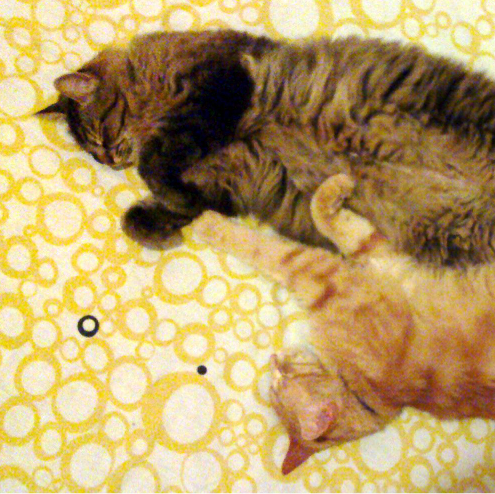
\includegraphics[width=0.9\marginparwidth]{figures/cats}
%     \caption{In this image, the cats are tessellated within a square
%       frame. Images should also have captions and be within the
%       boundaries of the sidebar on page~\pageref{sec:sidebar}. Photo:
%       \cczero~jofish on Flickr.}~\label{fig:marginfig}
%   \end{minipage}
% \end{marginfigure}


% \begin{figure*}
%   \centering
%   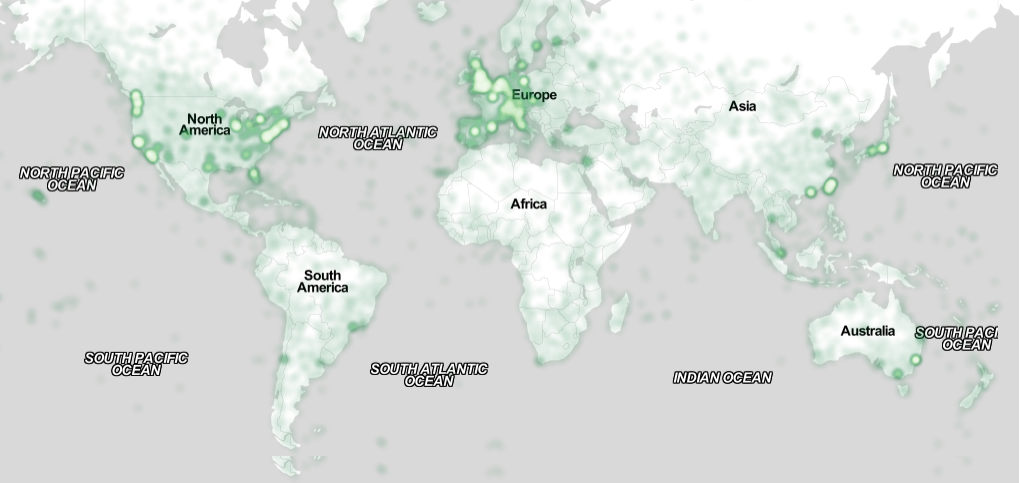
\includegraphics[width=1.3\columnwidth]{figures/map}
%   \caption{In this image, the map maximizes use of space. You can make
%     figures as wide as you need, up to a maximum of the full width of
%     both columns. Note that \LaTeX\ tends to render large figures on a
%     dedicated page. Image: \ccbynd~ayman on Flickr.}~\label{fig:cats}
% \end{figure*}

% \marginpar{\vspace{-23pc}So long as you don't type outside the right
%   margin or bleed into the gutter, it's okay to put annotations over
%   here on the left, too; this annotation is near Hawaii. You'll have
%   to manually align the margin paragraphs to your \LaTeX\ floats using
%   the \texttt{{\textbackslash}vspace{}} command.}

% \begin{margintable}[1pc]
%   \begin{minipage}{\marginparwidth}
%     \centering
%     \begin{tabular}{r r l}
%       & {\small \textbf{First}}
%       & {\small \textbf{Location}} \\
%       \toprule
%       Child & 22.5 & Melbourne \\
%       Adult & 22.0 & Bogot\'a \\
%       \midrule
%       Gene & 22.0 & Palo Alto \\
%       John & 34.5 & Minneapolis \\
%       \bottomrule
%     \end{tabular}
%     \caption{A simple narrow table in the left margin
%       space.}~\label{tab:table2}
%   \end{minipage}
% \end{margintable}


%%% Local Variables:
%%% mode: latex
%%% TeX-master: t
%%% End:
